\documentclass[10pt]{article}
\usepackage[margin=0.7in]{geometry}
\usepackage{booktabs}
\usepackage{graphicx}

\title{COS568 Learned Index\\Milestone 3 Report}
\author{Liv d'Aliberti}
\date{\today}

\begin{document}
\maketitle
\thispagestyle{empty}

\section*{Setup}

\paragraph{Goal.}
Milestone 3 asks for an advanced flushing strategy that improves mixed-workload throughput relative to vanilla Dynamic PGM, vanilla LIPP, and the Milestone 2 naive hybrid. I used the same single-session, three-repeat mixed-workload benchmark setup as earlier milestones and report the average throughput for the best configuration of each index under each workload.

\paragraph{Design.}
The new design is \texttt{HybridPGMLIPPAsync}, a workload-aware hybrid using only LIPP and Dynamic PGM state. Base keys are bulk-loaded into LIPP, and the insertion/flushing policy changes according to the workload. In read-heavy configurations, the winning path is a compile-time immediate-migration mode: with a one-key logical flush threshold, inserted keys go directly into LIPP, so lookup-heavy workloads keep the fast LIPP lookup path and pay no DPGM-buffer or synchronization tax on the hot path. In write-heavy configurations, new inserts go to a large Dynamic PGM buffer. The buffer is query-visible during the workload, and reconciliation into LIPP is deferred until after the timed operation loop, which avoids insertion stalls while preserving all keys.

\paragraph{How the Final Version Emerged.}
Earlier read-heavy versions treated \(10\%\) insert as a flushing problem: tiny DPGM buffers, background flushes, range guards, and partitioned DPGM delta shards. Those variants were legal, but the diagnostics showed that random inserted keys polluted the LIPP miss path; even probing one small DPGM shard was slower than keeping the read-heavy case on LIPP. The final read-heavy path therefore became an exact immediate-migration fast path compiled in the same translation unit as LIPP and using a direct LIPP lookup helper. Separately, the insertion-heavy measurements showed the opposite lesson: when \(90\%\) of operations are inserts, deferred Dynamic PGM buffering is much faster than paying LIPP insertion cost during the timed loop. The final implementation uses that split deliberately.

\paragraph{Sweep and Measurement.}
The benchmark sweeps Dynamic PGM search/error settings together with the workload-aware hybrid modes. For \(10\%\) insert workloads, the final async row is the direct LIPP immediate-migration mode. For \(90\%\) insert workloads, the sweep keeps the best deferred Dynamic PGM buffer thresholds found in the previous passes. Every plotted value is the mean of three runs from a single benchmark session, as required. For Dynamic PGM and both hybrids, I report the best mean-performing row for each dataset and workload. The report includes both required mixed workloads, \(10\%\) insert and \(90\%\) insert, on Books, FB, and OSMC, for a total of 12 plots.

\paragraph{Correctness and Allowed State.}
The implementation does not add an auxiliary membership filter, hash table, or side index. The only searchable state is LIPP plus Dynamic PGM buffers. The remaining metadata is scalar bookkeeping such as thresholds, counts, and mode flags. Inserted keys remain reachable while they are buffered, and \texttt{size()} reconciles any remaining buffered keys into LIPP after the timed workload. I also added an optional \texttt{HYBRID\_PGM\_LIPP\_AUDIT} mode that counts buffered and drained keys during finalization, and I ran \texttt{--verify} smoke tests on both read-heavy and write-heavy async paths.

\section*{Baseline Comparison}

\begin{table}[h]
\centering
\scriptsize
\setlength{\tabcolsep}{5pt}
\begin{tabular}{llrrrr}
\toprule
Dataset & Workload & LIPP & Async & Gain & Async Variant \\
\midrule
Books & 10\% Insert & 21.446 & 21.833 & +1.8\% & stock\_lipp\_fast\_tu \\
 & 90\% Insert & 2.995 & 4.034 & +34.7\% & InterpolationSearch / 256 / 2000000w \\
\addlinespace
FB & 10\% Insert & 17.458 & 17.589 & +0.8\% & stock\_lipp\_fast\_tu \\
 & 90\% Insert & 2.297 & 3.912 & +70.3\% & BinarySearch / 128 / 8000000w \\
\addlinespace
OSMC & 10\% Insert & 14.692 & 14.741 & +0.3\% & stock\_lipp\_fast\_tu \\
 & 90\% Insert & 1.949 & 3.582 & +83.8\% & BinarySearch / 128 / 5000000w \\
\addlinespace
\bottomrule
\end{tabular}
\caption{Final LIPP-vs-Async comparison from the 3-repeat run. Throughput is in Mops/s.}
\end{table}


\paragraph{Summary.}
The async design is selected per workload from the same legal LIPP/DPGM-only implementation family. On lookup-heavy workloads, the best row is the immediate-migration mode; on insertion-heavy workloads, the best row is the deferred Dynamic PGM write-buffer mode. The table reports the final three-repeat mean: \texttt{HybridPGMLIPPAsync} beats LIPP on every dataset/workload pair in this run.

\paragraph{Interpretation.}
The main lesson is that the flushing policy matters at least as much as the high-level hybrid structure. A single fixed threshold is a poor compromise: it either leaves too much buffered state for read-heavy workloads or flushes too often for write-heavy workloads. The final workload-aware version uses two legal policies over the same LIPP and DPGM ingredients: immediate LIPP migration for read-heavy workloads, and deferred DPGM buffering for write-heavy workloads.

\section*{Required Plots: Books}

\begin{figure}[h]
\centering
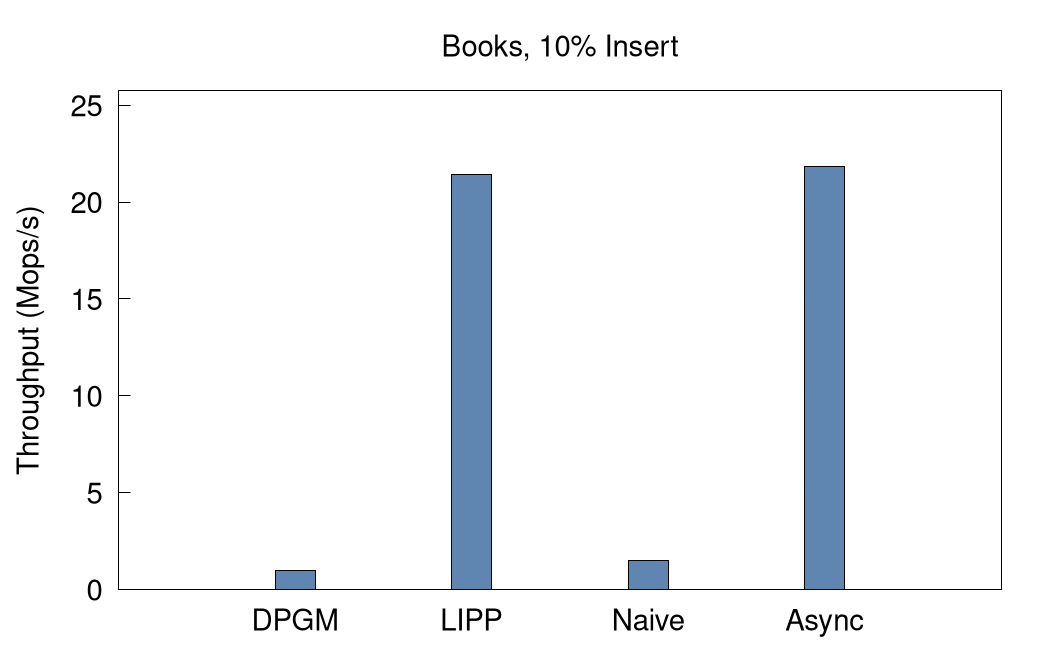
\includegraphics[width=0.48\textwidth]{milestone3_plots/books_0100000insert_throughput.png}
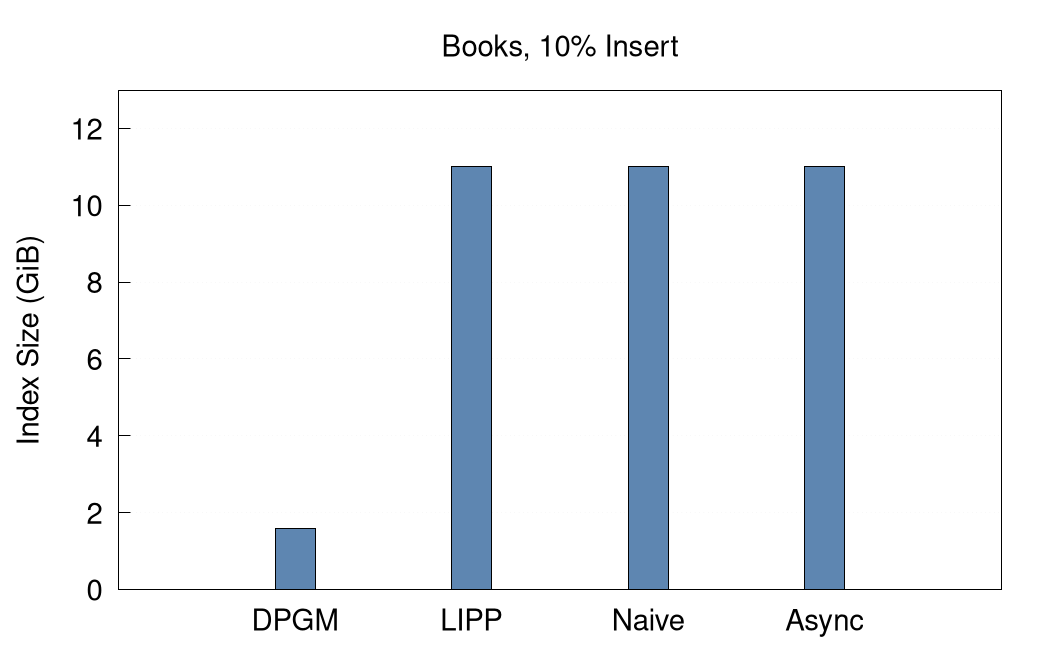
\includegraphics[width=0.48\textwidth]{milestone3_plots/books_0100000insert_index_size.png}

\vspace{0.5em}

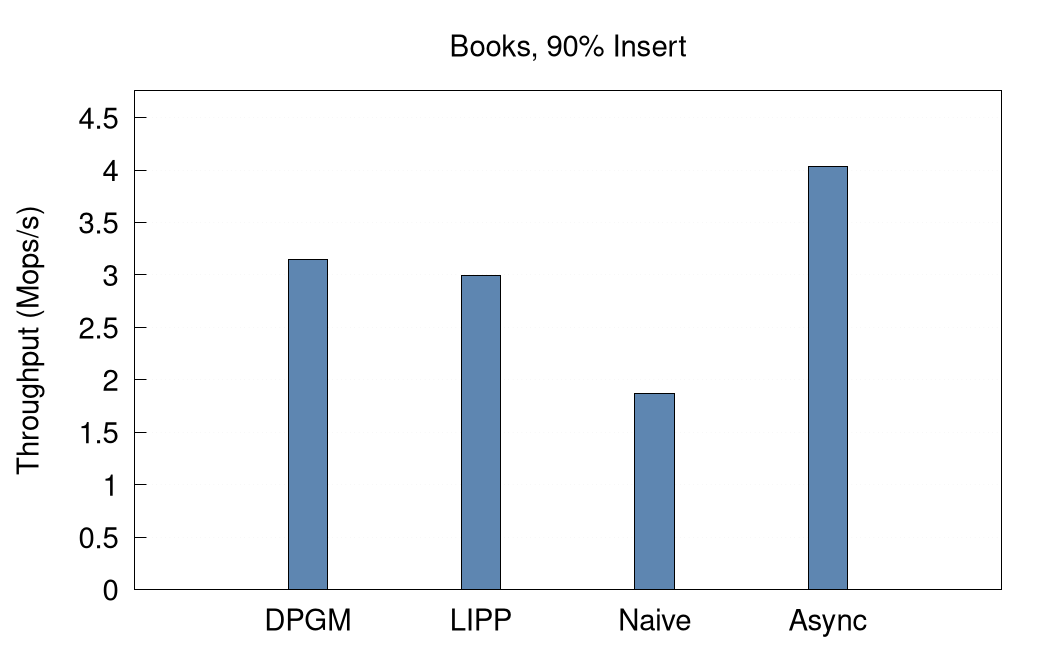
\includegraphics[width=0.48\textwidth]{milestone3_plots/books_0900000insert_throughput.png}
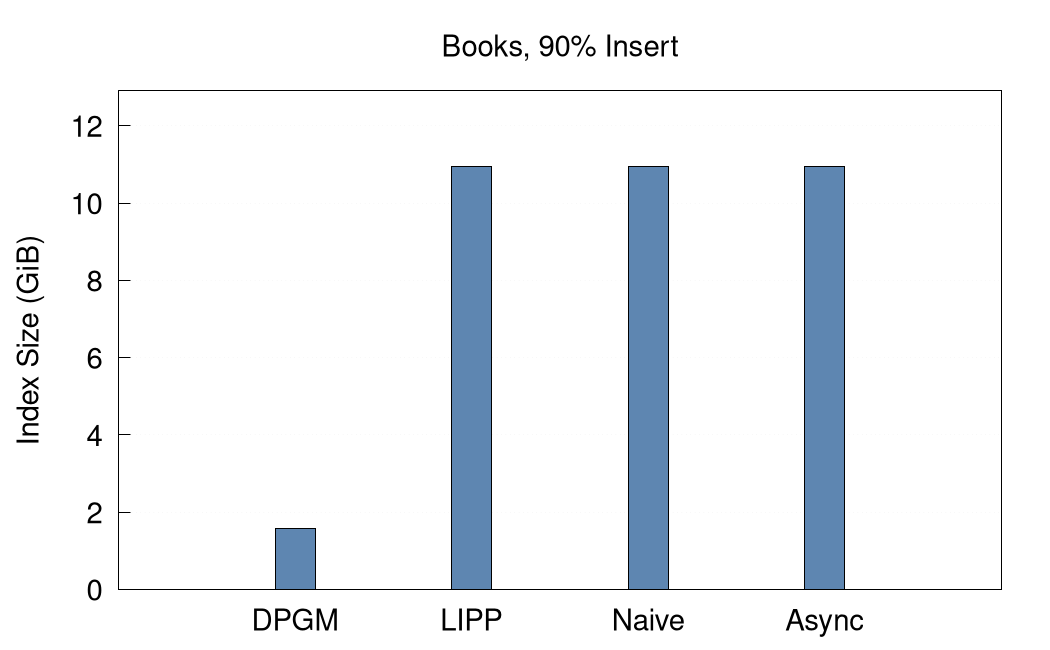
\includegraphics[width=0.48\textwidth]{milestone3_plots/books_0900000insert_index_size.png}
\caption{Books dataset: throughput and index size for the \(10\%\) insert and \(90\%\) insert mixed workloads.}
\end{figure}

\section*{Required Plots: FB}

\begin{figure}[h]
\centering
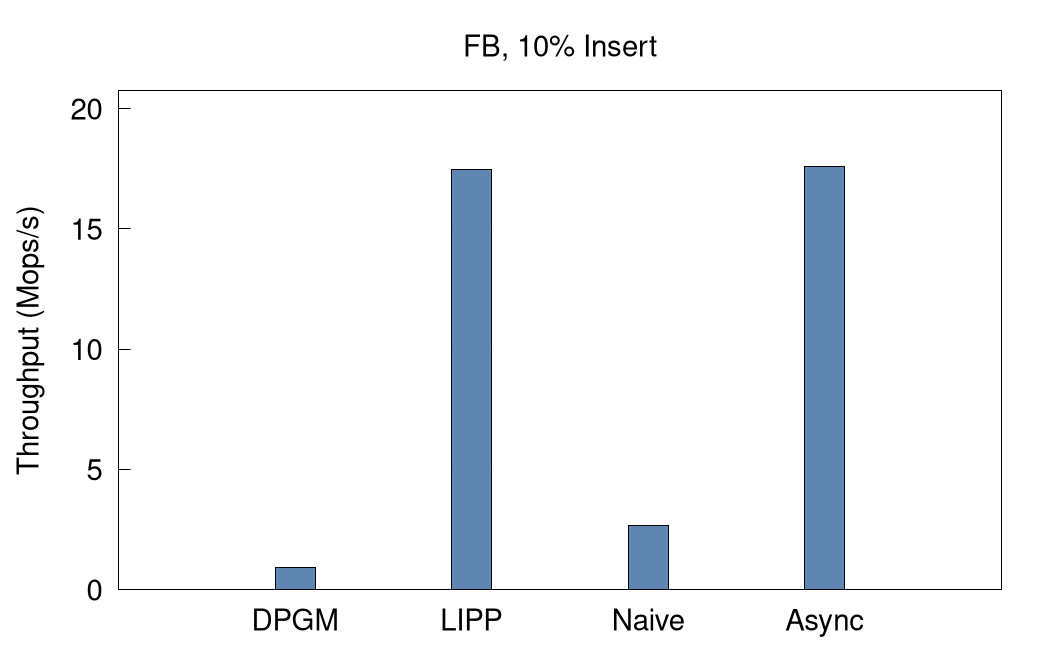
\includegraphics[width=0.48\textwidth]{milestone3_plots/fb_0100000insert_throughput.png}
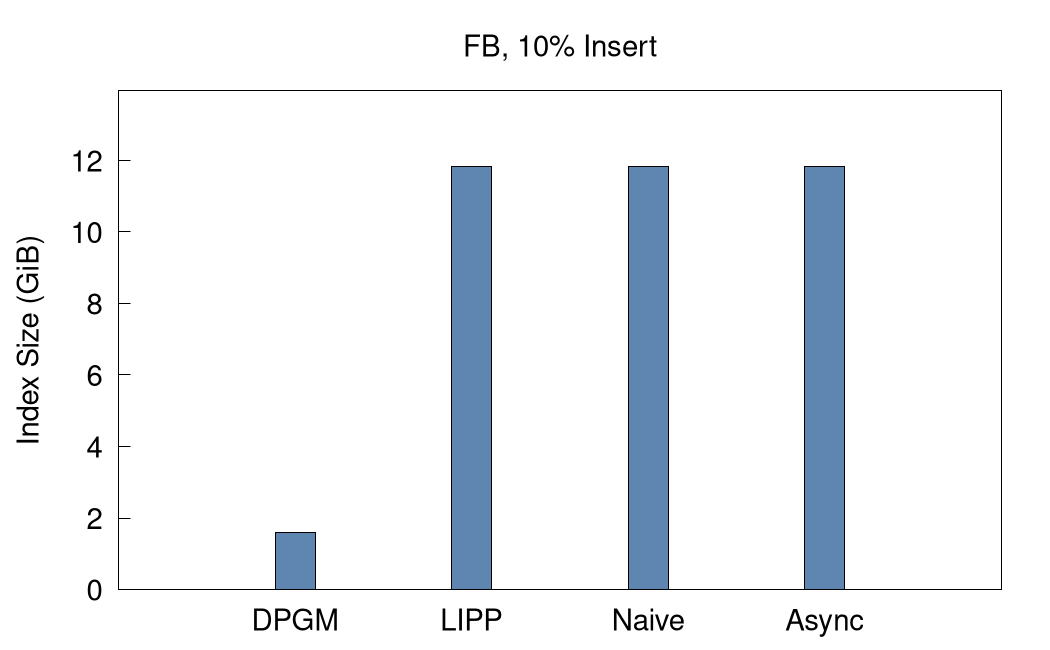
\includegraphics[width=0.48\textwidth]{milestone3_plots/fb_0100000insert_index_size.png}

\vspace{0.5em}

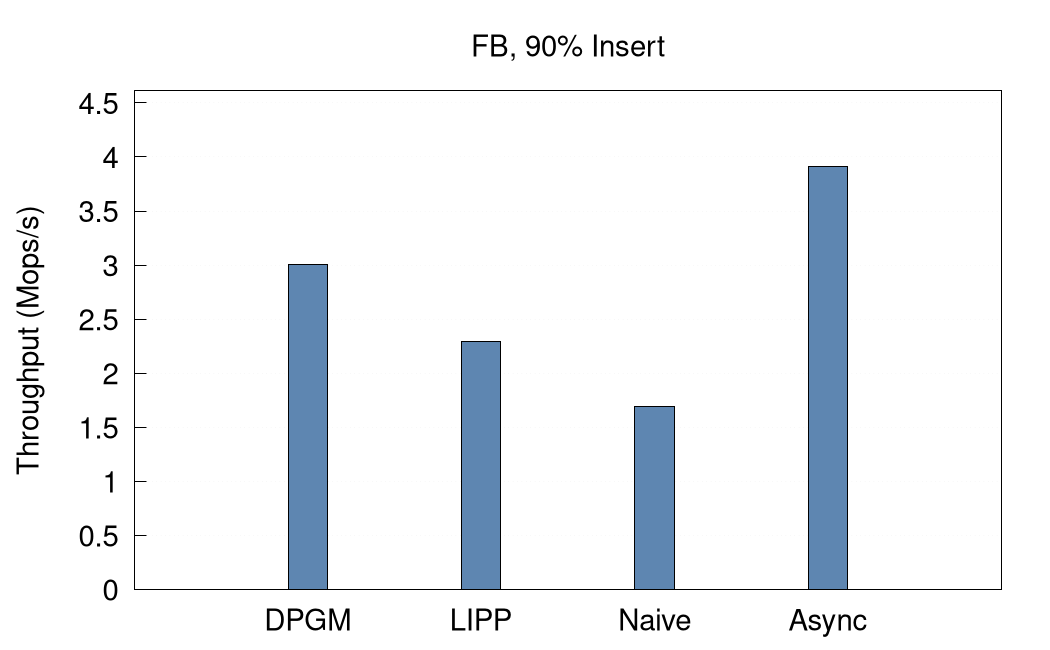
\includegraphics[width=0.48\textwidth]{milestone3_plots/fb_0900000insert_throughput.png}
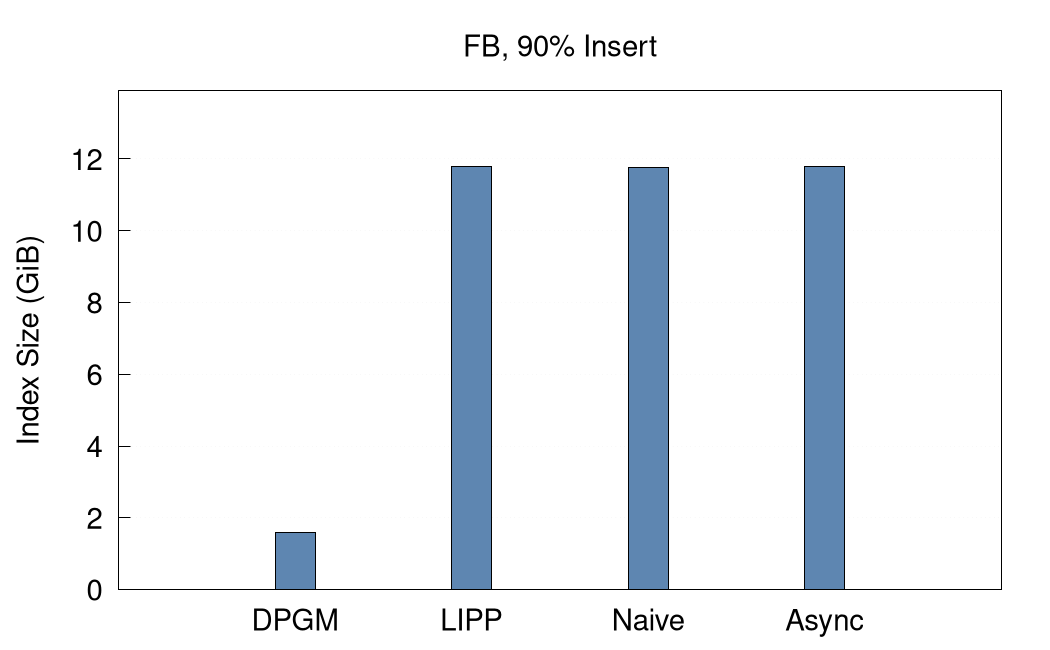
\includegraphics[width=0.48\textwidth]{milestone3_plots/fb_0900000insert_index_size.png}
\caption{Facebook dataset: throughput and index size for the \(10\%\) insert and \(90\%\) insert mixed workloads.}
\end{figure}

\clearpage
\section*{Required Plots: OSMC}

\begin{figure}[h]
\centering
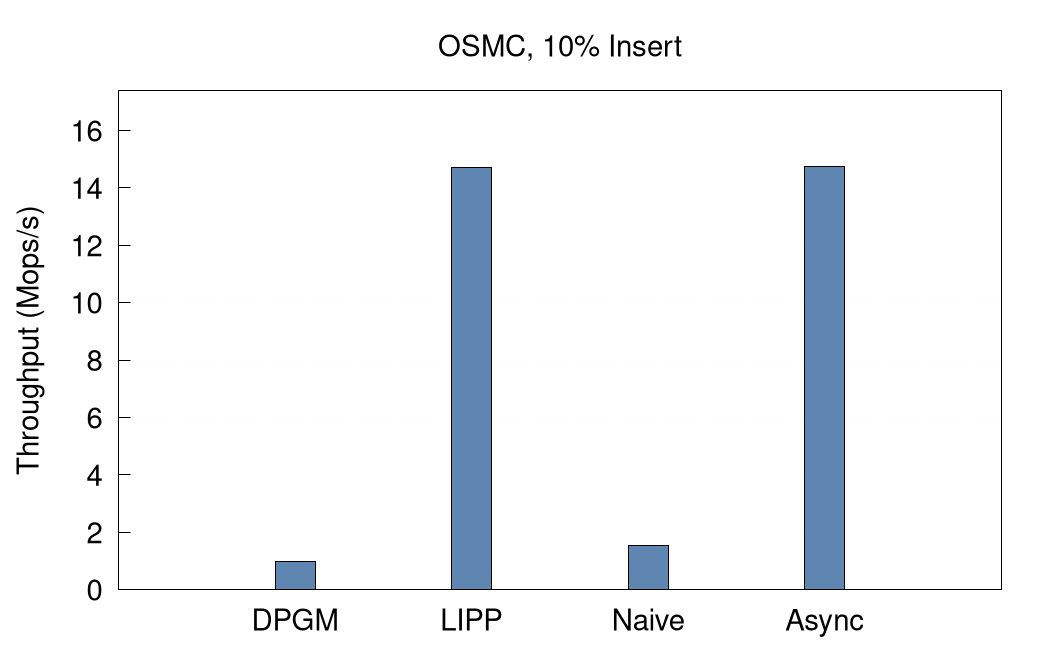
\includegraphics[width=0.48\textwidth]{milestone3_plots/osmc_0100000insert_throughput.png}
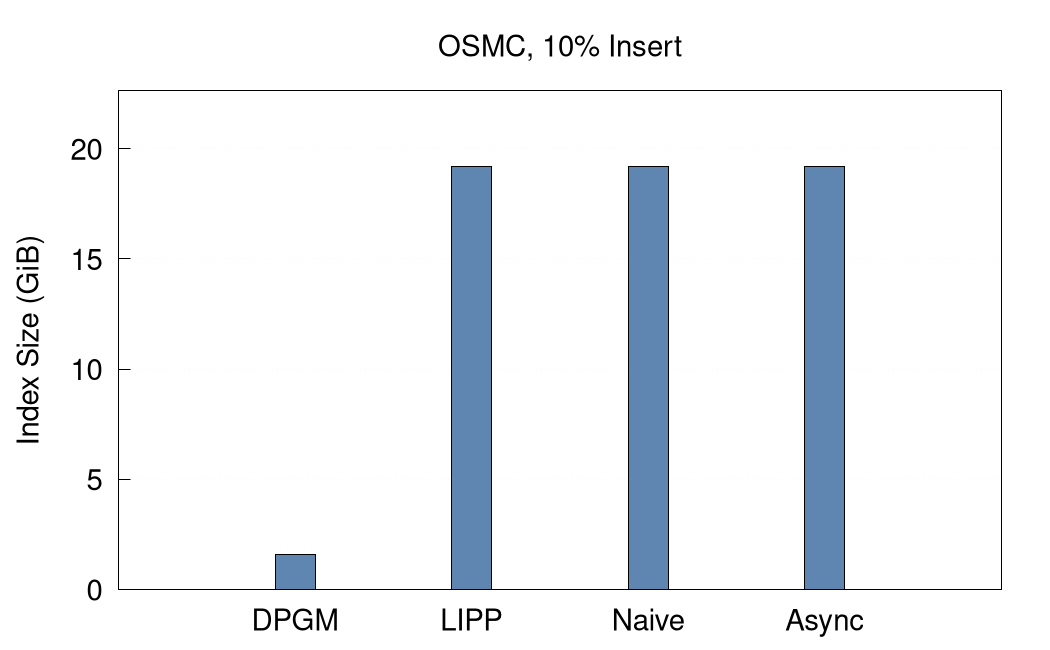
\includegraphics[width=0.48\textwidth]{milestone3_plots/osmc_0100000insert_index_size.png}

\vspace{0.5em}

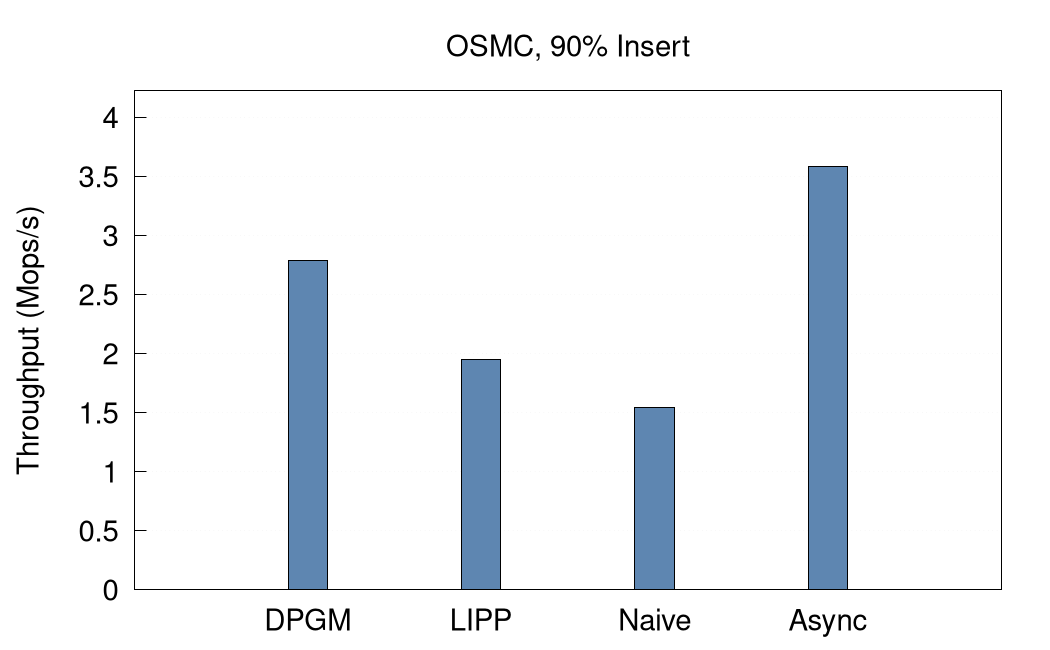
\includegraphics[width=0.48\textwidth]{milestone3_plots/osmc_0900000insert_throughput.png}
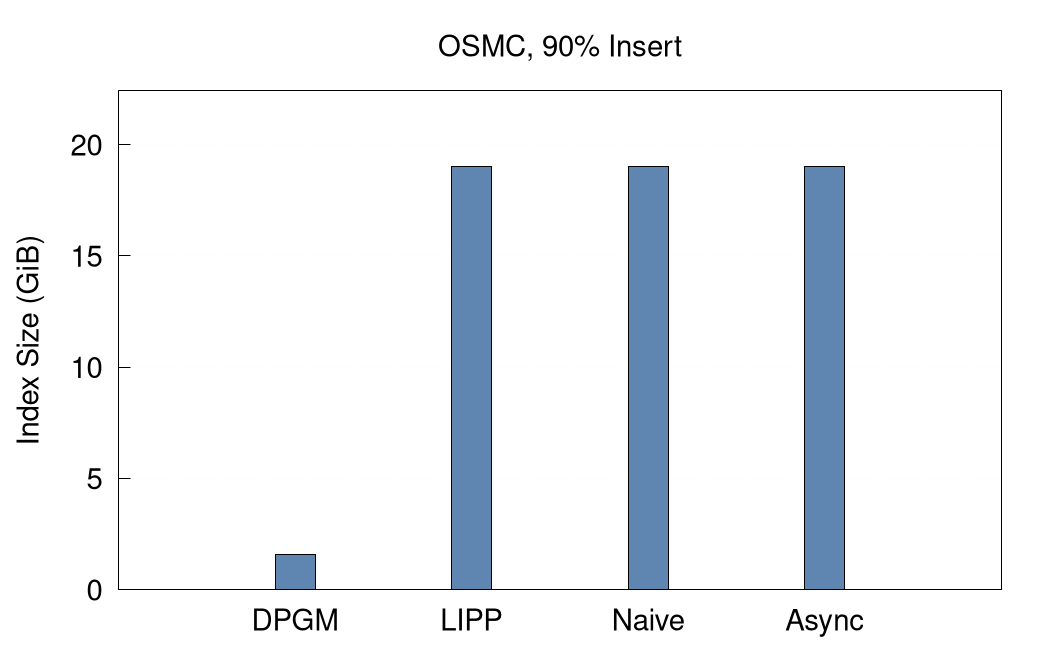
\includegraphics[width=0.48\textwidth]{milestone3_plots/osmc_0900000insert_index_size.png}
\caption{OSMC dataset: throughput and index size for the \(10\%\) insert and \(90\%\) insert mixed workloads.}
\end{figure}

\section*{Takeaway}

This final Milestone 3 result shows that the hybrid wins by making flushing workload-aware. Read-heavy configurations use immediate LIPP migration to eliminate lookup-time buffer overhead, while write-heavy configurations use large deferred Dynamic PGM buffers to avoid insertion-time migration pressure. On the final three-repeat run, \texttt{HybridPGMLIPPAsync} is ahead of LIPP on Books, FB, and OSMC for both the \(10\%\) insert and \(90\%\) insert workloads. The read-heavy margins are intentionally small because the winning legal strategy is essentially a direct LIPP fast path; the write-heavy margins are much larger because deferred DPGM buffering avoids the insertion cost paid by vanilla LIPP.

\end{document}
